\label{sec:testbed}

We proceed to define the testbed environment by each of its conforming
parts. We later indicate a procedure to set up the testbed. In this procedure,
we summarize all the details regarding on setting the connectivity and
system files for a set of \ac{Raspi}s in a centralized fashion.
Afterwards, we indicate how to cross-compile the Kodo library in an
easy way. Finally, we provide further information about Kodo itself in terms
of testing, other platforms supported and source code documentation
for further references.

\subsection{System Overview}


\begin{figure}[ht!]
\centering
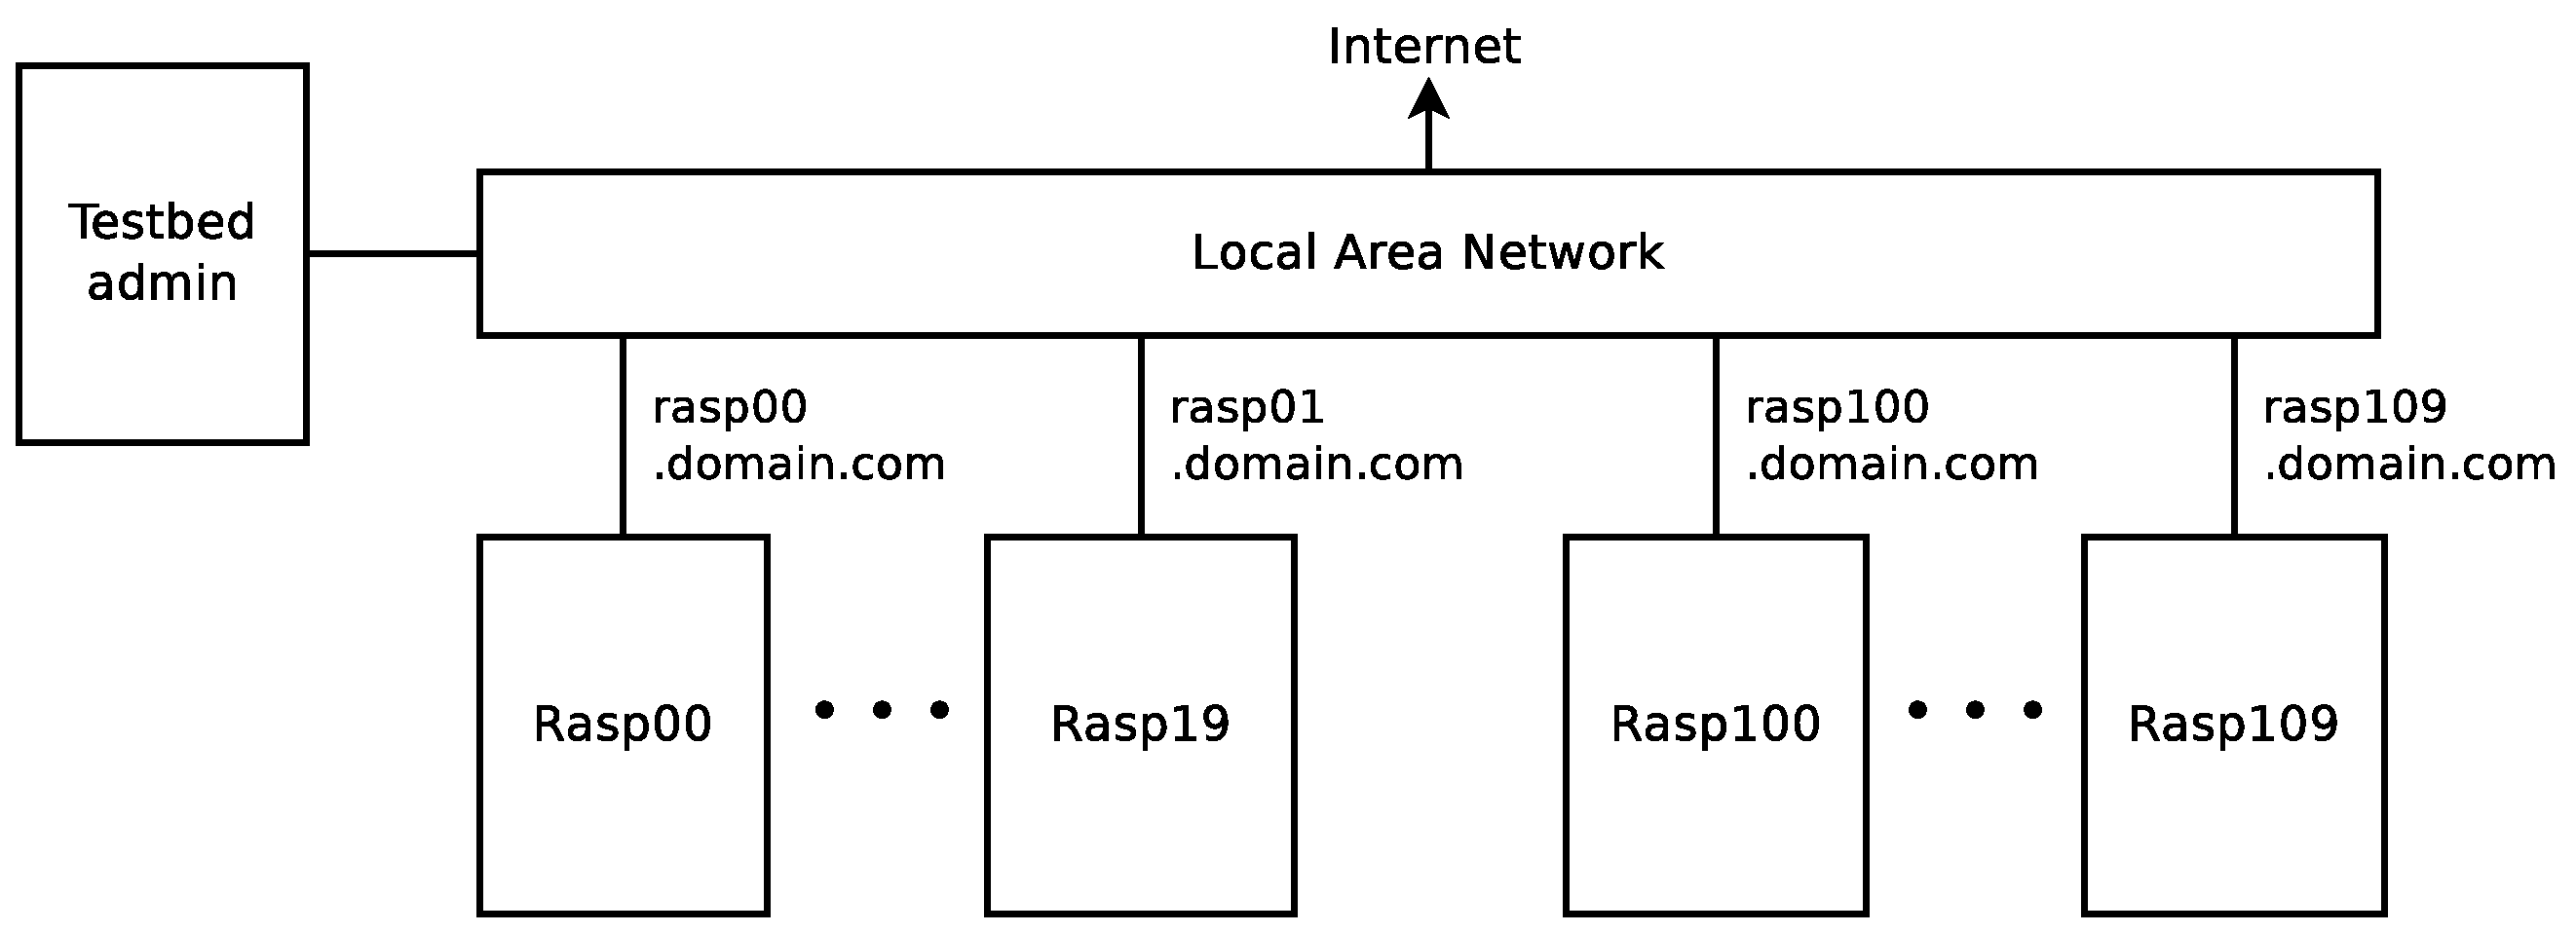
\includegraphics[width=0.6\textwidth]{images/testbed_setup2.eps}
\caption{Testbed setup}
\label{fig:testbed_setup}
\end{figure}

This section will present a testbed of thirty \ac{Raspi}s.
%Twenty \ac{Raspi} 1 model B revision 2 and ten \ac{Raspi} 2 model B V1.1.
They are all equipped with a memory card and are connected to the
university network by wire using their ethernet interface (eth0).

To easily discover the \ac{Raspi}s within the university network, they have all
been assigned a unique name under a common domain.
This eliminates the need to remember their individual \ac{IP}s.

A sketch of the testbed is depicted in figure~\ref{fig:testbed_setup}.
We have two types of \ac{Raspi}s in our setup.
Table \ref{tab:rasp_naming} shows the naming convention.

\begin{table}[ht!]
  \centering
  \begin{tabular}{|c|c|}
    \hline
      \textbf{Hostname} & \textbf{Model} \\ \hline
    Rasp00 - Rasp19 & Raspberry Pi 1 model B rev. 2 \\ \hline
    Rasp100 - Rasp109 & Rasperry Pi 2 model B V1.1 \\ \hline
  \end{tabular}
  \caption{Raspberry Pi naming convention}
  \label{tab:rasp_naming}
\end{table}




Accessing them is easily done using \ac{SSH}.
To address them within the university network,
The \ac{Raspi}s

The \ac{Raspi}s are all equipped with an ethernet interface (eth0) and
connected by wire to the university's \ac{LAN}. The university network
administration was provided
the \ac{MAC} addresses of the ethernet interfaces to automatically assign
the devices the desired \ac{IP} addresses as shown in the figure. In a personal
\ac{LAN}, another option could be to manually provide the devices with static
\ac{IP}s.


This section will be used to present a \ac{Raspi} testbed and the steps to
install and configure its devices.

The testbed is depicted in figure~\ref{fig:testbed_setup}. It consists of twenty
Raspberry Pi 1 model B rev 2 (Rasp01 to Rasp20) and
ten Raspberry Pi 2 model b V1.1 (Rasp2\_01 to Rasp2\_10).

The goal is to configure all the \ac{Raspi}s identically with the same software
and configurations. There are however a few differences between them that we
need to take into account. E.g. hostname and network addresses.

The testbed will be used by students that might need to change how the
devices are work either temporary or permanently. We will illustrate how this
can be accomplished using an overlaying filesystem.

Finally, it should be possible to store data that are generated from
simulations on the memory cards that are in the individual \ac{Raspi}.
%We using a overlaying filesystem that
%We will illustrate
%how that can be done. In the case of temporary changes, it is important that
%all changes can be easily reverted. We put a \ac{RAM} filesystem on top of
%the the root filesystem to .
%the configure the
%devices to behave according to their test specifications. We
%will also present how that might be done.

%their linkings. That could be to change network config

%The goal is to configure all the devices to be as identical as possible. This
%means that it is desired to have the same software on every device, but

The \ac{Raspi}s are all equipped with an ethernet interface (eth0) and
connected by wire to the university's \ac{LAN}. The university network
administration was provided
the \ac{MAC} addresses of the ethernet interfaces to automatically assign
the devices the desired \ac{IP} addresses as shown in the figure. In a personal
\ac{LAN}, another option could be to manually provide the devices with static
\ac{IP}s.
%that are
%assigned the \ac{IP} addresses in the figure and connected wired to the
%university's \ac{LAN}.

We use standard usb power adapters to power the \ac{Raspi}s.

\subsubsection{Installing Raspbian}

To get started, we first need to install an \ac{OS} on the
Raspberry Pis. We will use Raspbian linux~\cite{raspbian}

We will use a desktop that has linux installed to download,
configure, and write the image to the memory cards.
%We have decided to use a linux desktop machine to create a
%common image of Raspbian Linux that can be used in any of the Raspberry Pis.

%for all devices. After the image has been configured it can be written to
%a memory card and used in any of the Raspberry Pis. This means that each
%device needs a memory card, but it does not matter which card is put into
%which device.

We have decided to go with Raspbian linux~\cite{raspbian} and
to install it on memory cards.


%There exists a number of ways to setup a testbed in a centralized manner.
%E.g. using e.g. \ac{NFS}.

There exists a number of ways to setup a testbed

with multiple devices. We
have decided on a very simple approach of simply instal


-
- Download image (wget)
- Update/Modify image (chroot)
- Burn image
- Bang! linux is running
-

Open a terminal, and then...

hashmark (\#) means to perform operation as root, dollar (\$) means to perform operation as user


The first thing we need to do is to download the linux installation file.
For Raspbian, this is available at \url{http://downloads.raspberrypi.org}.

Raspbian is made available in two bundles. Raspbian and Raspbian lite.
The difference between the two is that Raspbian contains a pre-installed desktop
environment, and Raspbian lite is by default only accessable through a shell. 
They will both also be remotely accessible using \ac{SSH}.

Our testbed does not have monitors so we will install Raspbian lite.
A desktop environment can always be installed manually in case that will be
desired sometime in the future.

Below is a procedure of how we setup the \ac{Raspi}s in our testbed. We
have decided a simple setup where each \ac{Raspi} is equipped with a
memory card that contains a slightly customized Raspbian lite image with
identical settings. 

The reason this can be done easily is because the official Raspbian lite image
that we will download simply conntains a complete linux installation that are
packaged in an image rather than written to a harddrive, memory card, or usb
pen.

The overall steps to customize the official Raspbian lite image are listed below:
\begin{enumerate}
    \item Download Raspbian lite
    \item Alter Raspbian lite. E.g. browse, modify, add, and delete files
        in the official Raspbian lite image
    \item Change root. I.e. change root filesystem into the Raspbian lite
        image to update and install software packages
    \item Write image to memory cards
\end{enumerate}

\subsection{Download Raspbian lite}

To download the latest Raspbian lite, we go to the url
\url{http://downloads.raspberrypi.org/raspbian_lite/images/}.
At the time of this writing, the latest bundle was
2016-05-27-raspbian-jessie-lite.zip.

We want to proceed downloading the image with a shell instead of the browser.
To do this, first open a command window on a linux machine. This guide is
assuming a debian based distribution, but there should only be minor differences
if you have another package manager. I.e. the application that is used to
download and install software packages in linux.

After the terminal has been opened, we first declare a few variables to reduce
redundant typing. The first variables we declare is the Raspbian image name.
Notice that the extension has been omitted. This is because the image has been
packed into a zip file.
The other variable we declare is a working directory. This is where we will
download the image to and work on it. In other words, it will be stored in
/home/<username>/Raspbian

%To download Raspbian lite, we go to the \url{http://downloads.raspberrypi.org}.
%There should be a folder called raspbian\lite and
%to find the download page at which Raspbian lite should be located. Instead of
%downloading with the browser, we just extract the download url to the latest
%image. At the time of this writing, that was

% Define variable]
\begin{lstlisting}[]
$ export IMAGE="2016-05-27-raspbian-jessie-lite"
$ export WORKDIR="${HOME}/Raspbian"
\end{lstlisting}
\FloatBarrier

A final thing to notice is the way \$ and \# are used in the code blocks. \$
means that the command can be run as a normal user where \# indicates that the
command should be run with root permissions.
Running a command with root permissions can on most systems be done by putting
the command "sudo" in front of each line. This is illustrated in the code below
with the command "whoami" that prints the username of the caller. Lines without
leading \$ or \# is the terminal output.

% Root example
\begin{lstlisting}[]
$ whoami
chres
$ sudo whoami
root
\end{lstlisting}
\FloatBarrier

Next, we make the working directory and change directory (cd) into the working
directory. We can then use wget to download Raspbian lite. Unpack the image
when the download is complete.

% Download and unpack image
\begin{lstlisting}[]
$ mkdir -p ${WORKDIR}
$ cd ${WORKDIR}
$ wget http://downloads.raspberrypi.org/raspbian_lite/images/raspbian_lite-2016-05-31/${IMAGE}.zip
$ unzip ${IMAGE}.zip
\end{lstlisting}
\FloatBarrier

\subsection{Mount image}

After Raspbian lite has been unpacked, there should be an .img file in the directory.
"fdisk" can be used to display what is inside. Pass the arguments "-u sectors" to
display the sizes in sectors and "-l" to display partitions and exit.

% Check out the image   % The dollar hack was to fix vim syntax
\begin{lstlisting}[literate={DOLLAR}{\$}1]
DOLLAR fdisk -u sectors -l ${IMAGE}.img
Disk 2016-05-27-raspbian-jessie-lite.img: 1.3 GiB, 1387266048 bytes, 2709504 sectors
Units: sectors of 1 * 512 = 512 bytes
Sector size (logical/physical): 512 bytes / 512 bytes
I/O size (minimum/optimal): 512 bytes / 512 bytes
Disklabel type: dos
Disk identifier: 0x6fcf21f3

Device                               Boot  Start     End Sectors  Size Id Type
2016-05-27-raspbian-jessie-lite.img1        8192  137215  129024   63M  c W95 FAT32 (LBA)
2016-05-27-raspbian-jessie-lite.img2      137216 2709503 2572288  1.2G 83 Linux
\end{lstlisting}
\FloatBarrier

The image contains two partitions. The first one of starting at sector 8192 and
the other partition starting at sector 137216. The partitions is of type FAT32
and Linux and have sizes 63M and 1.2G. This indicates that the first partition
is most likely a boot partition and the second partition is a traditional file
system. Actually, it is a linux root filesystem (i.e. /).



%We see that the boot and root partitions starts at sector 8192 and 137216 respectivly.
%We also notice that each sector is 512 bytes.


%On newer systems, we can mount the device easier using "losetup --show -f -P IMAGE"

%Mount root partition:

To browser and alter the files in the image, it is possible to mount the partitions.

Lets first mount the root partition. This is done by first creating a new folder
that we will call root which will be located in our working directory. After this,
we mount the partition starting at sector 137216. To provide this offset information
to mount, we need to find the offset in bytes. From the fdisk command we could also
see that each sector is 512 bytes. Thus, we multiply the sector size and the sector
start to get the offset in bytes.

\begin{lstlisting}[]
$ export ROOTDIR="${WORKDIR}/root"
$ mkdir -p ${ROOTDIR}
# mount -o loop,offset=$((137216*512)) ${IMAGE}.img ${ROOTDIR}
\end{lstlisting}
\FloatBarrier

After this, we can also mount the boot partition inside the newly mounted
root filesystem. This is useful because that partition will be mounted
this exact place when a \ac{Raspi} starts up with a memory card containing
this image. It is therefore the natural place to mount it for later purposes.

Mount boot partition:
\begin{lstlisting}[]
# mount -o loop,offset=$((8192*512)) ${IMAGE}.img ${ROOTDIR}/boot
\end{lstlisting}
\FloatBarrier

We can now change all the files in the disk image as desired.



\subsection{Configuring OS files and scripts}

The \ac{Raspi}s should be setup to be as similar as possible. One of those
things that is prefered to be different on the devices is their hostname.
This helps distinguish them from each other. One solution to this in our
approach would be to uniquely change the hostname in each memory card.
This is however not desired because that would either require modifying
the the customized Raspbian lite image before writing the content to the
memory card or to manually change it in the \ac{Raspi}s after the image has
been written to a meomory card.
Instead, we decided to register the ethernet MAC addresses of all the \ac{Raspi}s
in our testbed. Those had to be used to put them in a domain name anyway.

Below is a part of the file where we keep track of the MAC addresses and assign
hostnames. This file will be available online and copied to the Raspbian lite
image in a later step under the listed filename. For different \ac{Raspi}s
the MAC addresses has to be changed. The MAC address of a network card can be found
using the command "ifconfig" or "ip addr".

% MAC and Hostname file
\Suppressnumber\begin{lstlisting}[]
<@\textcolor{gray}{\$\{ROOTDIR\}/home/pi/rasp\_config/nodes.csv}@>
<@\textcolor{gray}{
---------------------------------------------------------------}
\Reactivatenumber @>
# Ethernet MAC    Hostname
b8:27:eb:5b:da:20 rasp00
b8:27:eb:7b:c3:91 rasp01
b8:27:eb:54:9c:64 rasp02
b8:27:eb:95:bd:11 rasp03
\end{lstlisting}
\FloatBarrier

Provided that each \ac{Raspi} will have knowledge of all other \ac{Raspi}s in
the testbed, it still needs to know which name to give itself.
We do this using a small Bash script:

% Set hostname
\Suppressnumber\begin{lstlisting}[]
<@\textcolor{gray}{\$\{ROOTDIR\}/home/pi/rasp\_config/set\_hostname}@>
<@\textcolor{gray}{
---------------------------------------------------------------}
\Reactivatenumber @>
#!/usr/bin/env bash

script_path="$(dirname $(realpath $0))"
mac=$(cat /sys/class/net/eth0/address)
hostname=$(grep $mac ${script_path}/nodes.csv | cut -f2 -d' ')

# Assign hostname found in nodes.csv
if [ ! -z $hostname ]; then
    echo $hostname > /etc/hostname
    hostname $hostname
fi
\end{lstlisting}
\FloatBarrier

Line 1 tells the system to interpret the script using Bash. Line 3 gets the
path of the script itself. Line 4 gets the MAC address. This script will be
located in a \ac{Raspi} and thus return the MAC address of itself when called.
Line 4 searches line by line for this mac address.
Line 8-11 assigns the hostname found in "nodes.csv". If the MAC did not exists,
then it will keep the default hostname of the system.


We have packed the files and uploaded them to a webserver. These can be
retrieved with wget and unziped into the Raspbian lite image that
we are customizing:

% Get the files
\begin{lstlisting}[]
$ wget http://kom.aau.dk/project/TuneSCode/raspi/rasp_config.zip
# unzip rasp_config.zip -d ${ROOTDIR}/home/pi/
\end{lstlisting}
\FloatBarrier

"nodes.csv" can be changed using a text editor. For vim, this could be done
the following way:
\begin{lstlisting}[]
# vim ${ROOTDIR}/home/pi/rasp_config/nodes.csv
\end{lstlisting}
\FloatBarrier


Finally, to actually make the \ac{Raspi}s change hostname, we have to make
each \ac{Raspi} call the above script when it starts up.
Do this by inserting the line below in "\$\{ROOTDIR\}/etc/rc.local".
The file
can be opened with your favorite text editor.

\begin{lstlisting}[]
bash /home/pi/rasp_config/set_hostname"
\end{lstlisting}
\FloatBarrier


%This can be done by inserting a call to the script
%set\_hostname in rc.local before it exits.
%
%Call set\_hostname script at startup. We insert a line of code to call script in rc.local just after the initial comments (i.e. lines starting with \#).
%\begin{lstlisting}[]
%# line_number=$(egrep -n -m1 "(^[^#])|(^$)" ${ROOTDIR}/etc/rc.local | cut -d: -f1)
%# sed -i "${line_number}c bash /home/pi/rasp_config/set_hostname" ${ROOTDIR}/etc/rc.local
%\end{lstlisting}
%\FloatBarrier
%$ line="bash /home/pi/.rasp_config/set_hostname"
%# awk -v text="$line" '!/^#/ && !p {print text; p=1} 1' ${ROOTDIR}/etc/rc.local > <@ \Suppressnumber @>
%    ${ROOTDIR}/etc/rc.local <@ \Reactivatenumber @>

All other files could be updated as well.

\subsection{Installation and Updating the image}

It may be desired to pre-install some programs in the image before it is
written to all the memory cards that goes into the \ac{Raspi}s.
This can be done from any linux x86 machine using QEMU Chroot (change root).
\url{https://wiki.debian.org/QemuUserEmulation}
%\url{https://wiki.archlinux.org/index.php/Raspberry_Pi}

Due to the \ac{ARM} processor that \ac{Raspi}s are using, it is required to
install some additional software:
%Because \ac{Raspi}s are eqipped with an \ac{ARM} processor 
%%it is not as
%straightforward as performing the task for two linux systems of the same
%architecture.

% CHROOT to OS image
\begin{lstlisting}[]
# apt-get install binfmt-support qemu qemu-user-static
# update-binfmts --display qemu-arm
qemu-arm (enabled):
     package = qemu-user-static
        type = magic
      offset = 0
       magic = \x7fELF\x01\x01\x01\x00\x00\x00\x00\x00\x00\x00\x00\x00\x02\x00\x28\x00
        mask = \xff\xff\xff\xff\xff\xff\xff\x00\xff\xff\xff\xff\xff\xff\xff\xff\xfe\xff\xff\xff
 interpreter = /usr/bin/qemu-arm-static
    detector = 
\end{lstlisting}
\FloatBarrier
% This was neccessary on arch
%# update-binfmts --importdir /var/lib/binfmts/ --import

Make sure the second command writes "enabled" as the output above. If that 
is not the case, then try enabling it:

\begin{lstlisting}[]
# update-binfmts --enable qemu-arm
\end{lstlisting}
\FloatBarrier

Provided that qemu-arm is enabled, we should now be able to change root (chroot)
into our Raspbian lite image. Change root is a method i linux that enables
the root (/) to be changed. Thus, enabling a linux installation within a
linux installation.

There are a few commands to be performed before we can change root.
First, to get internet access from within the Raspbian lite image it is needed
to copy our resolv.conf into the filesystem. Line 1 steps into Raspbian lite's
root filesystem. Then line 2 copies resolv.conf.

% CHROOT to OS image
\begin{lstlisting}[]
# cd $ROOTDIR
# cp /etc/resolv.conf etc/resolv.conf
\end{lstlisting}
\FloatBarrier

Now, because of the ARM architecture, it is also required to copy
/usr/bin/qemu-arm-static into the image before we can continue:

% CHROOT to OS image
\begin{lstlisting}[]
# cp /usr/bin/qemu-arm-static usr/bin
\end{lstlisting}
\FloatBarrier

The final preparation before chaning root is to populate the directories proc,
sys, and dev:

% CHROOT to OS image
\begin{lstlisting}[]
# mount -t proc proc proc/
# mount --rbind /sys sys/
# mount --rbind /dev dev/
\end{lstlisting}
\FloatBarrier

Finally, the filesystem is ready for us to change root. This can be done with
"proot". It may be required to install proot:

% CHROOT to OS image
\begin{lstlisting}[]
# proot -q qemu-arm-static -S ${ROOTDIR}
\end{lstlisting}
\FloatBarrier

Most available online material uses the more known chroot command as written in
the code block below. This did not work correctly in our machines, but we show
it as an alternative in case proot may not work on other systems.

% CHROOT to OS image
\begin{lstlisting}[]
# chroot ${ROOTDIR} /usr/bin/qemu-arm-static /bin/bash    (ALTERNATIVE TO proot)
\end{lstlisting}
\FloatBarrier

If everything went well, we should now be standing in the Raspbian lite filesystem
under its root. Optionally, we can change the prompt title to indicate that we
are chrooted:

% Optionally, we may create a unique prompt to indicate we have changed root
\begin{lstlisting}[]
# export PS1="(chroot) $PS1"
\end{lstlisting}
\FloatBarrier

The Raspbian lite system should now be possible to use as if it had been booted
in a \ac{Raspi}. The only difference is that the laptop that we are using is
significantly faster than a \ac{Raspi}. Thus enabling us to for example update,
upgrade, and install software packages:

% Update system
\begin{lstlisting}[]
# apt-get update
# apt-get upgrade
\end{lstlisting}
\FloatBarrier

Lets install some useful applications:
% Install packages
\begin{lstlisting}[]
# apt-get install vim git screen
\end{lstlisting}
\FloatBarrier

All the changes that are made here will exists in all \ac{Raspi}s when the
image is written to a memory card.

\subsection{Installation an overlaying filesystem}

Our goal was to enable the users of the testbed to change however the
\ac{Raspi} are configured while still being able to revert those changes easily.

We do this by storing a users work in the \ac{Raspi}s in \ac{RAM}. Thus a
\ac{Raspi}, when a \ac{Raspi} is rebooted, it will forget all changes.

A way to do this is using stacked filesystem. Stacking filesystem enables
a filesystem to overlay another filesystem. Whenever a file is accessed,
the upper filesystem will forward the request to the lower filesystem in
case it does not have it itself. If it has it, it will simpy return the file.

This idea can be used in our setup to mount the root filesystem (i.e. Raspbian
lite) in the \ac{Raspi}s duing startup as read-only. Thus, the files will not
be changable. Some programs needs to change files and the testbed admin might
want to change configurations. To enable this, it is possible to
overlay a filesystem that is mounted in \ac{RAM} as read/writable on top of
the regular root. Thus, reading a file may return a file from the lower filesytem,
but if it is stored, it will be saved in the upper filesystem. Accessing this file
again will return the stored file from the upper layer.



%We do this using an overlay filesystem. The idea is to let the \ac{Raspi}s
%mount their root filesystem as 
%
%We do this using an overlay filesystem (overlayfs).
%Overlayfs enables a filesystem to be stacked on top of another filesystem. Thus,
%if the \ac{Raspi}s mount their root filesystem (/) as read-onlyif we mount our root (/) filesystem as 
%
%
%Overlayfs enables filesystems
%to be stacked on top of each other. We will be using this to make a lower
%filesystem and an upper filesystem. The lower filesystem will be our
%traditional filesystem and the upper filesystem will be mounted in tmpfs
%(i.e. mounted in \ac{RAM}).
%
%Thus, when a file is requsted from stacked filesystem, it will first attempt
%to fetch the file in the upper filesystem if it does not exists there, it will
%request it from the lower filessytem.  

Assuming that you are still chrooted into the Raspbian lite filesystem, we
can setup the overlay filesystem (overlayfs).

There already exists implementations overlaying the root filesystem. We will
use an existing implementation
available at github: \url{https://github.com/chesty/overlayroot}.

We installed git in a previous step, so lets clone the repository. The below
code stores it in /tmp which is really mounted in \ac{RAM}. Thus, the files
will disappear when the machine is rebooted.

% Get files
\begin{lstlisting}[]
# OVERLAYROOTDIR="/tmp/overlayroot"
# git clone https://github.com/chesty/overlayroot.git $OVERLAYROOTDIR
\end{lstlisting}
\FloatBarrier

To enable the overlaying filesystem it is required to generate an initial \ac{RAM}
file system (initramfs). Initramfs is an initial filesystem that gets loaded into
\ac{RAM} during the startup process of a linux machine to prepare the real
filesystem.

For this purpose, we need BuxyBox:

% Install required packages
\begin{lstlisting}[]
# apt-get install busybox
\end{lstlisting}
\FloatBarrier

Add and activate the overlaying filesystem, we need to add the scripts and tell initramfs
to load the overlaying filesytem:

% Setup initramfs
\begin{lstlisting}[]
# cp ${OVERLAYROOTDIR}/hooks-overlay /etc/initramfs-tools/hooks/
# cp ${OVERLAYROOTDIR}/init-bottom-overlay /etc/initramfs-tools/scripts/init-bottom/
# echo "overlay" > /etc/initramfs-tools/modules
\end{lstlisting}
\FloatBarrier

Raspbian lite uses a "u-boot" to boot, so it should be made aware of the
initramfs that we will generate.

% Tell uboot to load initramfs
\begin{lstlisting}[]
# echo "initramfs init.gz" > /boot/config.txt
\end{lstlisting}
\FloatBarrier

Finally, lets generate the image. This is done using "mkinitramfs", that will
by default look for the kernel modules of the current system. Remember we are
chrooted, so we need to specify the correct kernel modules to look for. These
can be found in "/lib/modules".

% Create an initramfs
\begin{lstlisting}[]
# ls /lib/modules/
\end{lstlisting}
\FloatBarrier

For \ac{Raspi} 1, our kernel modules was "4.4.11+". The other modules in /lib/modules
is for \ac{Raspi} 2.

Thus, to run mkinitramfs, type in the correct kernel version:

% Create an initramfs
\begin{lstlisting}[]
# mkinitramfs -o /boot/init.gz -k 4.4.11+
\end{lstlisting}
\FloatBarrier

This should generate a new initial \ac{RAM} filesystem that will overlay a \ac{RAM} filesystem.

\subsection{Write image}

The final step is to write the image to all the memory cards before they can
be plugged in the \ac{Raspi}s. This is done by first leaving the chrooted filesystem
and unmounting all the directories we mounted:

% Exit chroot, umount, and write to memory card
\begin{lstlisting}[]
# exit
# cd ..
# umount --recursive ${ROOTDIR}
# losetup -d WHICH_NUMBE.img
\end{lstlisting}
\FloatBarrier

If successfully unmounted, you can insert a memory card in your machine. In our
system, this memory card was available under /dev/mmcblk0, but this may be
different on different machines. For internal memory card readers, it will
probably be named /dev/mmcblkX where X is some number and if the memory card
reader is connected through \ac{USB}, then it is likely called /dev/sdX.
Make sure to write to the correct device as everything will be overwritten!

Below is a few commands that may help you to deduce which device is correct:

\begin{lstlisting}[]
# lsblk
# df -h
\end{lstlisting}
\FloatBarrier

For us, the device was /dev/mmcblk0, so we write the image to that device:
\begin{lstlisting}[]
# dd if=${IMAGE}.img of=/dev/mmcblk0 bs=4M
\end{lstlisting}
\FloatBarrier


\subsection{Kodo python}


\subsection{fabric}

% Exit chroot, umount, and write to memory card
\begin{lstlisting}[]
from fabric.api import run, env, task
# Python Fabric script to run commands on multiple hosts through ssh
#
# Run script as 'fab <task>', where <task> is one of the scripts functions
# marked as a tesk. The task marked as 'default' will be run if <task> is not
# specified

env.hosts = ['rasp00.domain.com','rasp01.domain.com','rasp02.domain.com']
env.user = 'root'
env.password = 'sdn'

@task
def install(program):
    """
    Install a program
    program: program name
    """
    result = run('apt-get install -y {}'.format(program), quiet=True)

@task
def copy_to_rasp(filename):
    put(...)

\end{lstlisting}
\FloatBarrier

execute a script function by calling "fab install:feh"

\section{Cross-compilation: From PC to Raspberry Pi}

%\subsection{Kodo cross-compilation: From your PC to the Raspberry Pi}

\subsection{Install toolchain on PC}

Besides the previous description (\textbf{Include compiling Kodo from the
RasPi from the scratch}), the testbed administrator can compile Kodo in its
personal workstation and transfer the generated binaries directly to
a path in the \ac{Raspi}. To achieve this, we get a toolchain that
contains the binaries for the \texttt{raspberry-gxx49-arm-g++} compiler
for the \ac{Raspi}. Therefore, we strongly recommend any testbed
administrator to do the following procedure. In what follows, we provide
the instructions considering that the NFS server uses the \texttt{\$HOME}
directory as the working directory. However, the administrator may choose
some other working directory of its preference if desired.

\begin{enumerate}

\item Create toolchain directory:
\begin{lstlisting}[]
$ TOOLCHAINDIR="${HOME}/toolchains"
$ mkdir -p $TOOLCHAINDIR
$ cd $TOOLCHAINDIR
\end{lstlisting}
\FloatBarrier
\vspace{-5mm}

\item Download the \ac{Raspi} toolchain for 64-bit Linux from.
A more recent \ac{Raspi} toolchain may be available at
\texttt{http://buildbot.steinwurf.dk/toolchains/linux/}:

\begin{lstlisting}[]
$ TOOLCHAIN="raspberry-gxx49-arm"
$ wget http://kom.aau.dk/project/TuneSCode/raspi/${TOOLCHAIN}.zip
\end{lstlisting}
\FloatBarrier
\vspace{-5mm}

\item Extract the downloaded file:
%locally in the NFS server. After
%this operation, there should be a new directory for the toolchain
%in the server. \\
\begin{lstlisting}[]
$ unzip ${TOOLCHAIN}.zip
\end{lstlisting}
\FloatBarrier
\vspace{-5mm}

\item (Optional) Delete zip file:
%locally in the NFS server. After
%this operation, there should be a new directory for the toolchain
%in the server. \\
\begin{lstlisting}[]
$ rm ${TOOLCHAIN}.zip
\end{lstlisting}
\FloatBarrier
\vspace{-5mm}

\item We can now verify that the ARM cross compiler is working:

\begin{lstlisting}[]
$ ${TOOLCHAINDIR}/${TOOLCHAIN}/bin/${TOOLCHAIN}-g++ --version
raspberry-gxx49-arm-g++ (crosstool-NG 1.21.0) 4.9.3 20150311 (prerelease)
Copyright (C) 2014 Free Software Foundation, Inc.
This is free software; see the source for copying conditions.  There is NO
warranty; not even for MERCHANTABILITY or FITNESS FOR A PARTICULAR PURPOSE.
\end{lstlisting}
\FloatBarrier
\vspace{-5mm}

%\begin{lstlisting}[]
%$ echo "${TOOLCHAINDIR}/${TOOLCHAIN}/bin/${TOOLCHAIN}-g++"
%/home/<USER>/toolchains/raspberry-gxx49-arm/bin/raspberry-gxx49-arm-g++
%\end{lstlisting}
%\FloatBarrier
%\vspace{-5mm}
    
%    The ARM cross compilers should now be located in

\item Make toolchain binaries available systemwide. Instead of calling
the ARM cross compiler using its full path, we can make it accessible
from the command shell systemwide. One way to do this is by adding the 
toolchain binaries directory to the Linux environment variable \texttt{PATH}
when the \ac{OS} starts up:

%\item Add toolchain binaries to \texttt{PATH}. Instead specifying the full
%path to the toolchain binaries we can instead tell the operation system
%where to search for it. This makes the toolchain binaries available
%systemwide.

\begin{lstlisting}[]
$ echo PATH=\"\$PATH:${TOOLCHAINDIR}/${TOOLCHAIN}/bin\" >> ${HOME}/.profile
\end{lstlisting}
\FloatBarrier
\vspace{-5mm}
%$ printf 'PATH="%s/%s/bin"\n' "${TOOLCHAINDIR}" "${TOOLCHAIN}" >> ${HOME}/.profile

%\item Add the \texttt{bin} folder of the toolchain to the \texttt{PATH}
%Linux environment variable of the server. This will help the server OS
%to recognize the location of the compiler command, which will be needed
%later. To do so, edit the \texttt{\$HOME/.profile} to add in a newline:
%\texttt{PATH="\$PATH:\$HOME/raspberry-gxx49-arm/bin"}. Save the
%\texttt{\$HOME/.profile}. \\

\texttt{.profile} should now contain the line we inserted. There may be more
code in you file.
% MAC and Hostname file
\Suppressnumber\begin{lstlisting}[]
<@\textcolor{gray}{\$HOME/.profile}@>
<@\textcolor{gray}{
---------------------------------------------------------------}
\Reactivatenumber @>
PATH="$PATH:/home/<USERNAME>/toolchains/raspberry-gxx49-arm/bin"
\end{lstlisting}
\FloatBarrier

\item Update \texttt{PATH}. Source \texttt{.profile} to make the changes
take effect in your system:
\begin{lstlisting}[]
$ source ${HOME}/.profile
\end{lstlisting}
\FloatBarrier
\vspace{-5mm}

\item ARM cross compiler should now be available systemwide:

\begin{lstlisting}[]
$ raspberry-gxx49-arm-g++ --version
\end{lstlisting}
\FloatBarrier
\vspace{-5mm}

%\item Restart the server session in order for the changes made in the
%previous step take effect. To verify this, open a new terminal and type:
%\texttt{raspberry-gxx49-arm-g++ --version}. A correct binary installation
%should return an output similar to:
%
%\texttt{raspberry-gxx49-arm-g++ (crosstool-NG 1.21.0) 4.9.3 20150311 (prerelease)
%Copyright (C) 2014 Free Software Foundation, Inc.
%This is free software; see the source for copying conditions.  There is NO
%warranty; not even for MERCHANTABILITY or FITNESS FOR A PARTICULAR PURPOSE.} \\

\end{enumerate}

\subsection{Cross compile example}

Create a directory to hold our code:
\begin{lstlisting}[]
$ CODEDIR="${HOME}/code"
$ mkdir -p ${CODEDIR}
$ cd ${CODEDIR}
\end{lstlisting}
\FloatBarrier
\vspace{-5mm}

Create a \texttt{hello\_world.cpp} using your favorite text editor:

\Suppressnumber\begin{lstlisting}[]
<@\textcolor{gray}{\${CODEDIR}/hello\_world.cpp}@>
<@\textcolor{gray}{
---------------------------------------------------------------}
\Reactivatenumber @>
#include <iostream>

int main()
{
    std::cout << "Hello World!" << std::endl;
    return 0;
}
\end{lstlisting}
\FloatBarrier

Save \texttt{hello\_world.cpp} and compile it for \ac{Raspi}:

\begin{lstlisting}[]
$ raspberry-gxx49-arm-g++ hello_world.cpp -o hello_world
\end{lstlisting}
\FloatBarrier
\vspace{-5mm}

Lets copy the executable file to a \ac{Raspi} and test it. We will use \ac{SCP}
to copy the executable to one of the \ac{Raspi}s.

Default username is "pi" and password is "raspberry"

\begin{lstlisting}[]
$ scp main pi:<RASP_IP>:~/
\end{lstlisting}
\FloatBarrier
\vspace{-5mm}

If you do not know the \ac{IP} address of a \ac{Raspi} in your network, you can
connect a monitor to it and run the following command after you have logged in:
\begin{lstlisting}[]
pi@rasp01:~ $ ifconfig
eth0      Link encap:Ethernet  HWaddr b8:27:eb:72:77:54  
          inet addr:192.168.87.107  Bcast:192.168.87.255  Mask:255.255.255.0
          inet6 addr: fe80::e0a5:38f3:6f82:bc79/64 Scope:Link
          UP BROADCAST RUNNING MULTICAST  MTU:1500  Metric:1
          RX packets:1537 errors:0 dropped:0 overruns:0 frame:0
          TX packets:445 errors:0 dropped:0 overruns:0 carrier:0
          collisions:0 txqueuelen:1000 
          RX bytes:259117 (253.0 KiB)  TX bytes:52551 (51.3 KiB)

\end{lstlisting}
\FloatBarrier
\vspace{-5mm}

After the executable has been copied to a \ac{Raspi}. Then, \ac{SSH} to it:

\begin{lstlisting}[]
$ ssh pi:<RASP_IP>
\end{lstlisting}
\FloatBarrier
\vspace{-5mm}

We can list the directory content after we have logged into the \ac{Raspi} and
see that \texttt{hello\_world} is there:

\begin{lstlisting}[]
pi@rasp07:~ $ ls
hello_world  rasp_config
\end{lstlisting}
\FloatBarrier
\vspace{-5mm}

Now, simply execute the \texttt{hello\_world}:

\begin{lstlisting}[]
pi@rasp07:~ $ ./hello_world
Hello World!
\end{lstlisting}
\FloatBarrier
\vspace{-5mm}

\subsection{Long running jobs over SSH (PUT THIS SECTION SOMEWHERE ELSE)}

Problem when you logout, then applications will terminate. SCREEN is the answer.

EXAMPLE

\texttt{hello\_world} returns immediately. This is not always the case.
Sometimes it is desired to run simulations that should run for days. 
A software package called \texttt{screen} can be used for this purpose.
Simply run ...

\subsection{Cross compile Kodo}

\begin{enumerate}

\item Clone the Kodo repository in the server by executing: \\
\texttt{git clone git://github.com/steinwurf/kodo.git} in \texttt{\$HOME}.
\textbf{Change the repo to kodo-rlnc or kodo-cpp since just raw kodo is going
to be depreceated soon} \\

\item Navigate to the repository and configure \texttt{waf} by typing:
\texttt{python config.py} and select the 16th ``make specification'' file
for the \ac{Raspi}, e.g. option \texttt{[16]cxx\_raspberry\_gxx49\_arm}
presented by the file.

This command configures \texttt{waf} to use the proper compiler and its
required flags to generate the binaries for the \ac{Raspi}. If the
configuration was correct, the output will indicate:
\texttt{'configure' finished successfully (X.XXXs)}, where \texttt{X.XXX}
is total time in seconds for configuring the project in the server. \\

\item Execute \texttt{python waf build}. If the build process was
successful, the generated binaries for the \ac{Raspi} should be located
in \texttt{build/cxx\_raspberry\_gxx49\_arm} in the Kodo repository.
\textbf{Indicate how the binary files should look like}.

Once this procedure is made, the testbed administrator can relocate the
generated binary files to the \ac{Raspi}s through the network as desired
by using the \texttt{scp} command during the configuration step.


\end{enumerate}

\subsection{Kodo Builds for the \ac{Raspi}, Platform Support and Documentation}

You can check the build status of Kodo, Fifi and other relevant projects
through their respective repository master branch on our buildbot page
\cite{steinwurf2016buildbot}. Our buildbot displays the status of the builds
for Raspbian 8 and GCC 4.9 for the ARM architecture which is the relevant one
for the \ac{Raspi}. At the link, you can check build status and build
statistics. Also, documentation about Kodo basics with a tutorial is available
at \cite{kododocs}.
